%!TEX root = ../paper.tex
\begin{figure}[!ht]
\centering
\noindent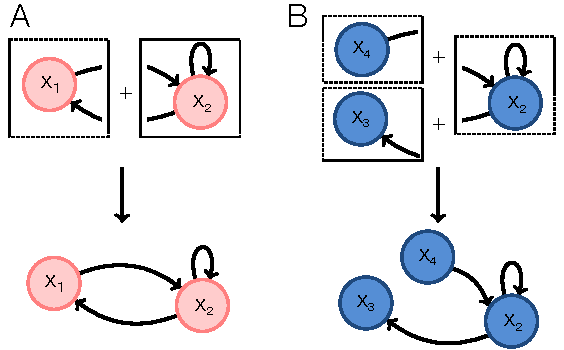
\includegraphics[width=0.4\columnwidth]{fig/examplesystemmodules.pdf}
\caption{{\bf Example of the combination of open system modules to construct closed systems.} (A) Example of combining two open modules to construct a closed system of two components (B) Analogous example for combining three open modules to construct a closed system with three components}
\label{fig:examplesystemmodules}
\end{figure}

\begin{figure}[!ht]
\centering
\noindent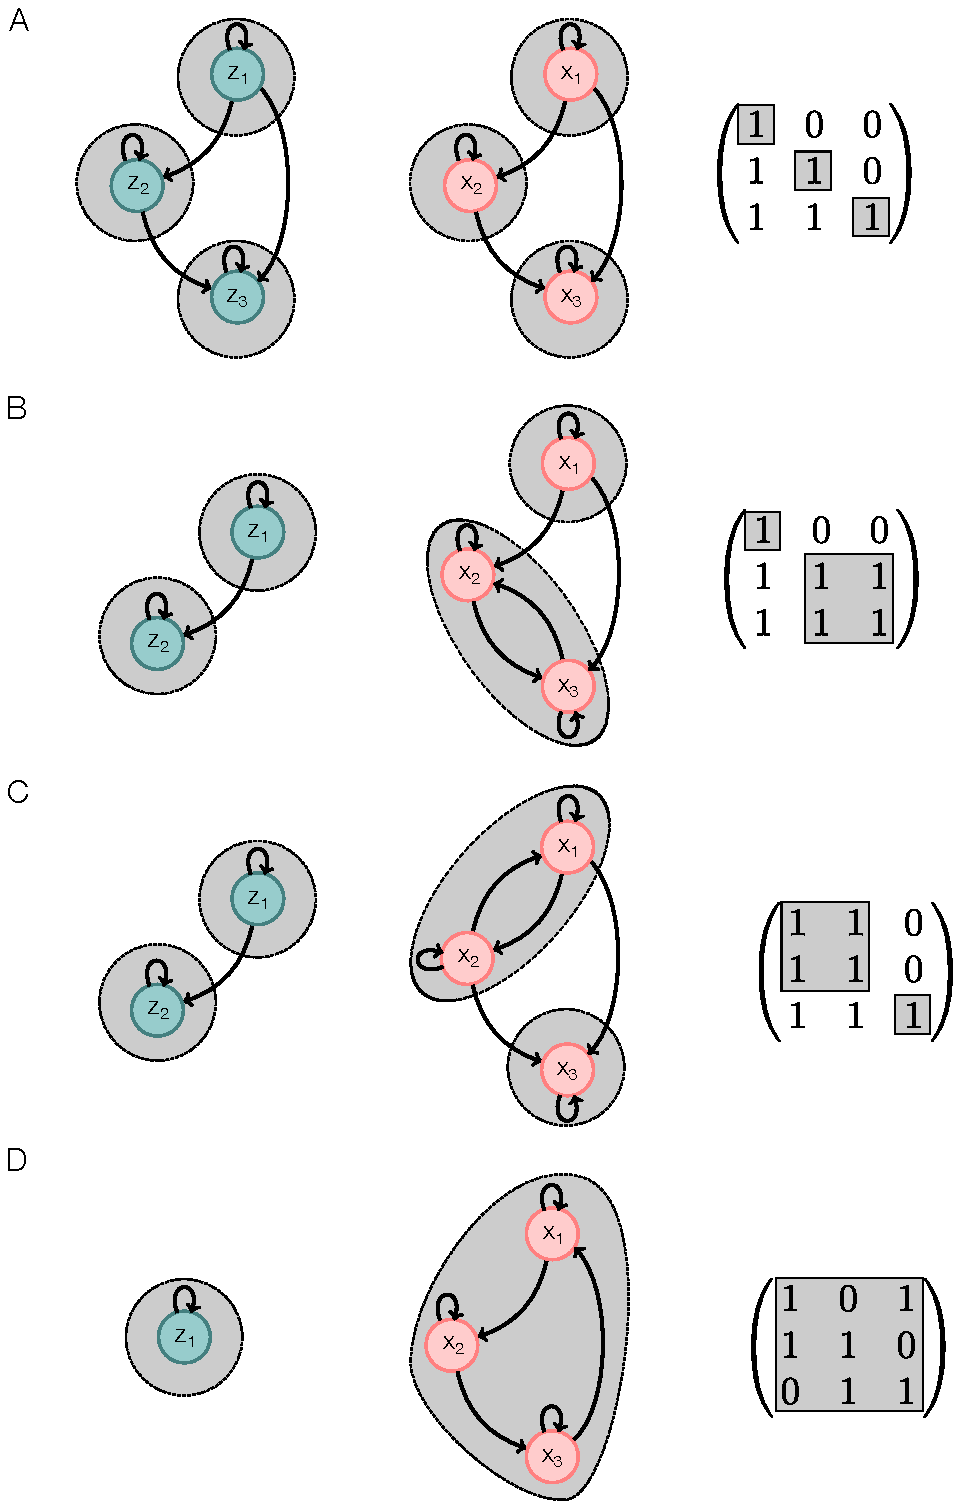
\includegraphics[width=0.5\columnwidth]{fig/scc2.pdf}
\caption{{\bf Example of strongly connected components.} (A) - (D) show strongly connected components highlighted in gray for each of the four graphs representing the interdependencies relevant to four different three component systems. Note that the most hierarchical system in (A) has the highest possible number of connected components, three, whereas the system containing a single cycle and therefore posessing no hierarchy contains only one connected component. Systems (B) and (C) represent examples of hierarchical modular systems that posess both modularity and hierarchy.}
\label{fig:scc}
\end{figure}

\begin{figure}[!ht]
\centering
\noindent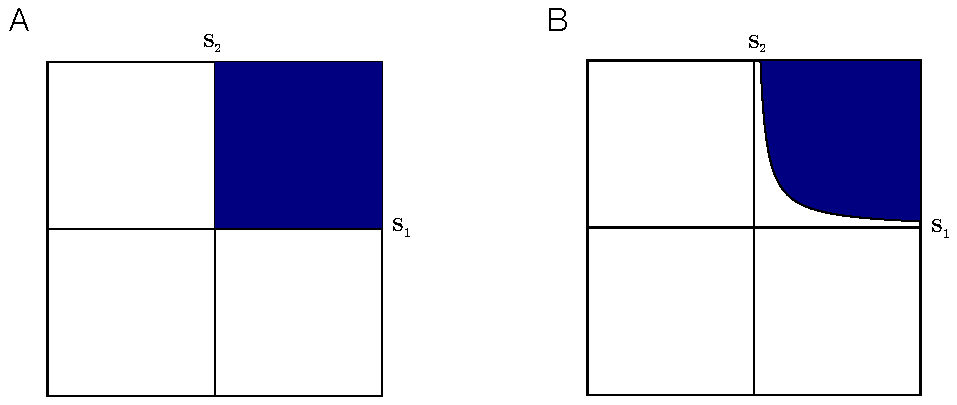
\includegraphics[width=0.8\columnwidth]{fig/region2and3.pdf}
\caption{{\bf Stability conditions on coefficients of the characteristic polynomial for two and three component systems.} The regions correspond to all possible relationships between the invariants determined by the characteristic polynomial.}
\label{fig:region2and3}
\end{figure}

\begin{figure}[!ht]
\centering
\noindent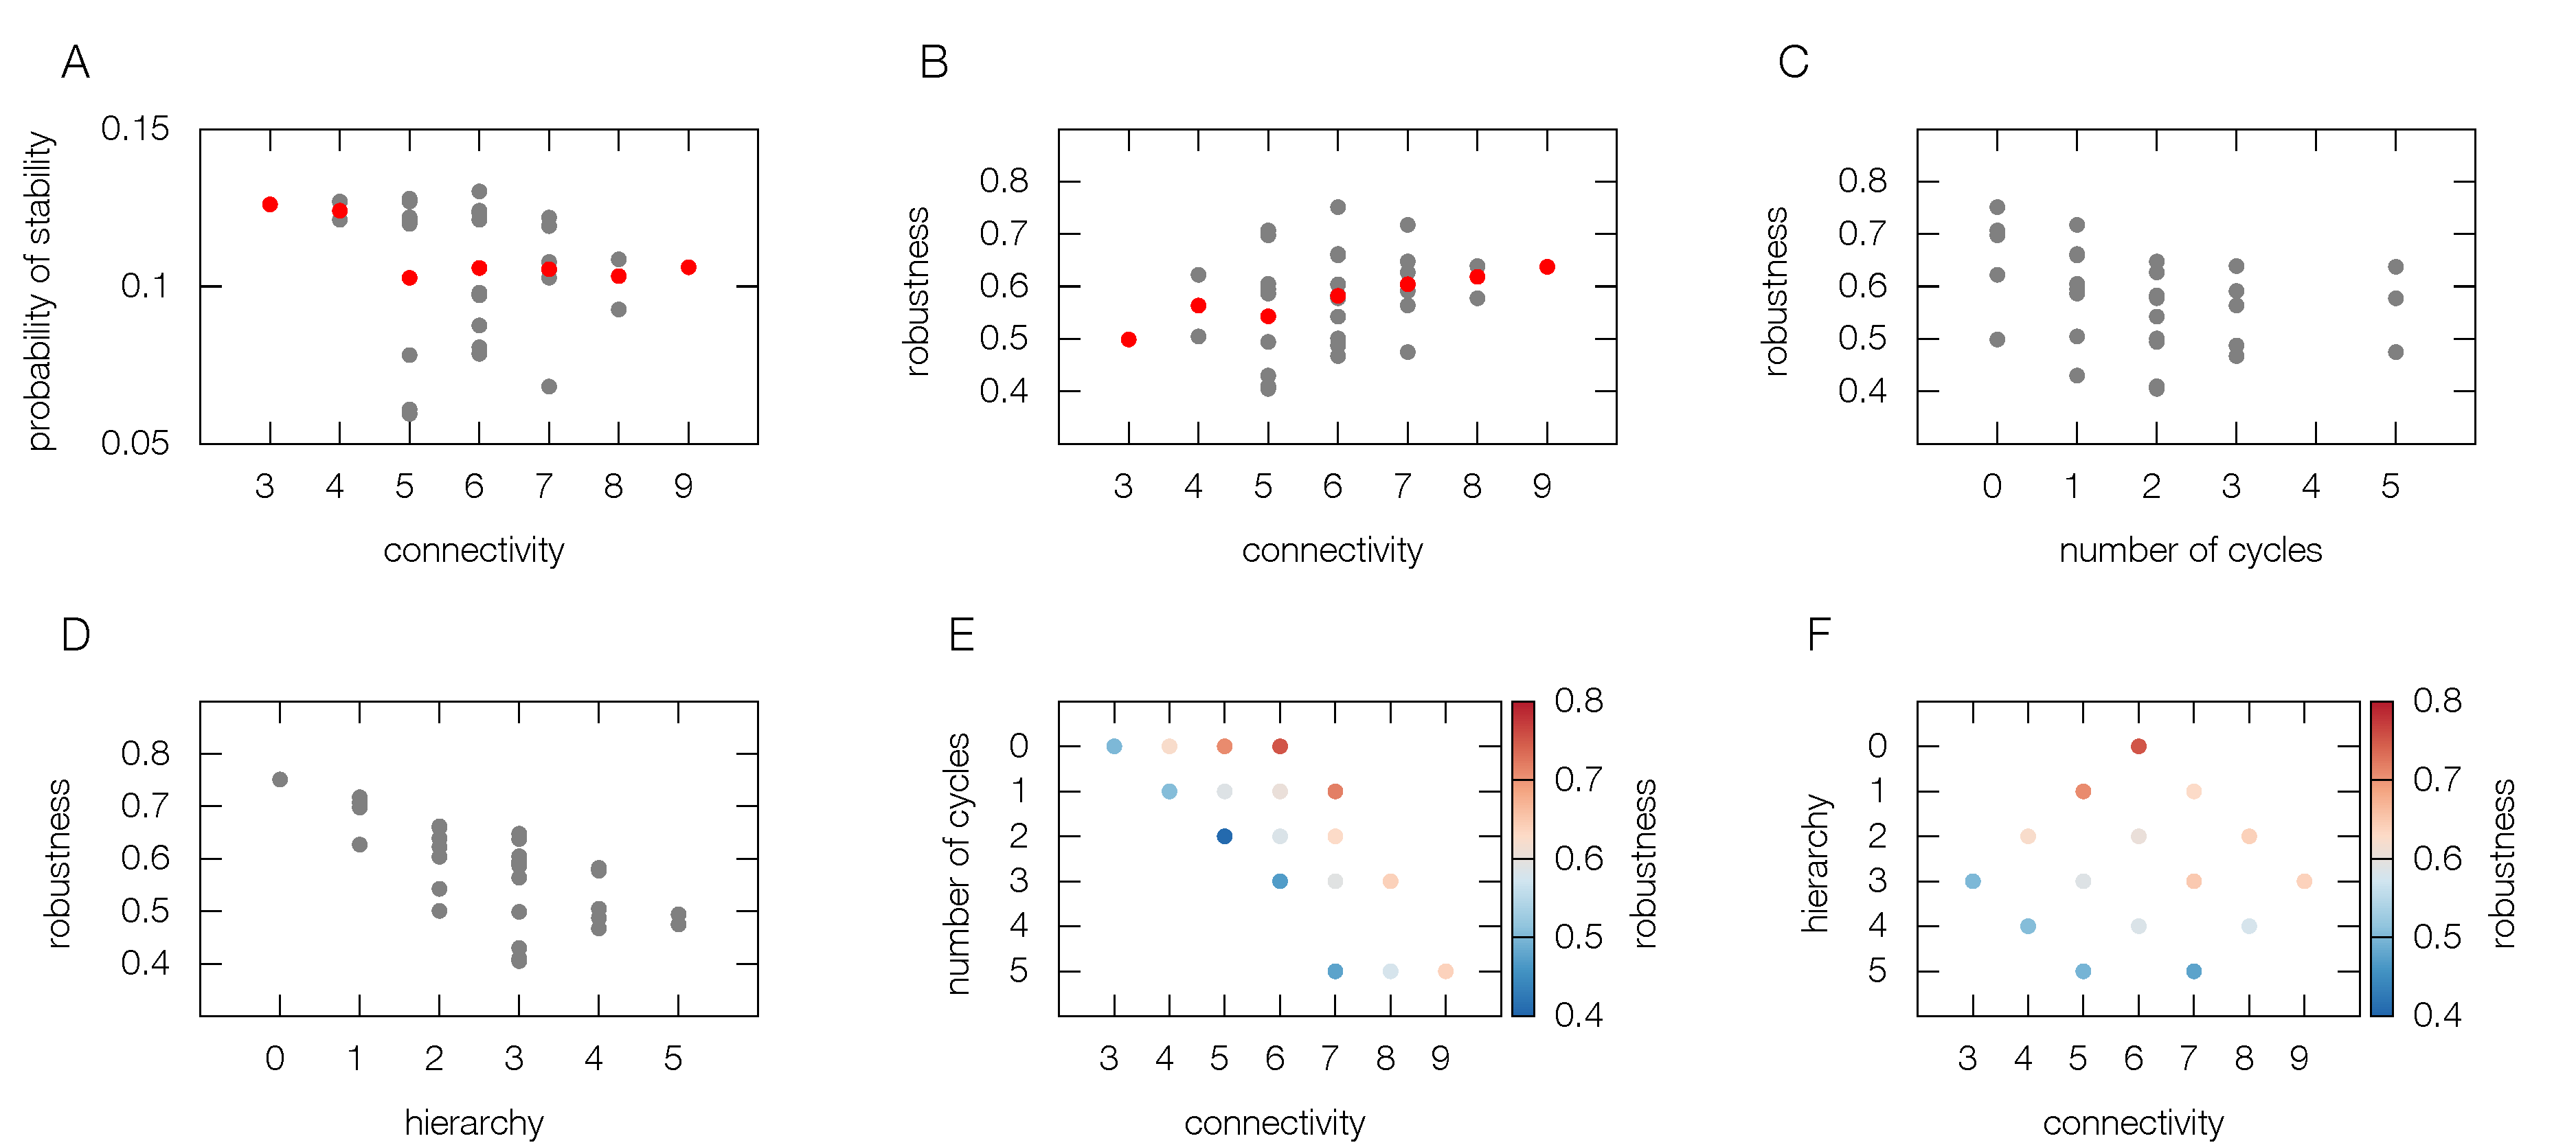
\includegraphics[width=1.0\columnwidth]{fig/combinedfigs.pdf}
\caption{{\bf Characterization of stability and robustness according to properties of system structure} (A) Stability versus connectivity, (B) robustness versus connectivity, (C) robustness versus number of cycles, (D) robustness versus graph edit distance, (E) robustness versus number of cycles and connectivity, and (F) robustness versus graph edit distance and connectivity for three component systems.}
\label{fig:combined}
\end{figure}

% Figure translations
% apstab3x3 4 -> A
% stab3x3 6 -> B
% cycle3x3 7 -> C
% New -> D
% connectcycle3D3x3 5 -> E
% New -> F

% \begin{figure}[!ht]
% \centering
% \noindent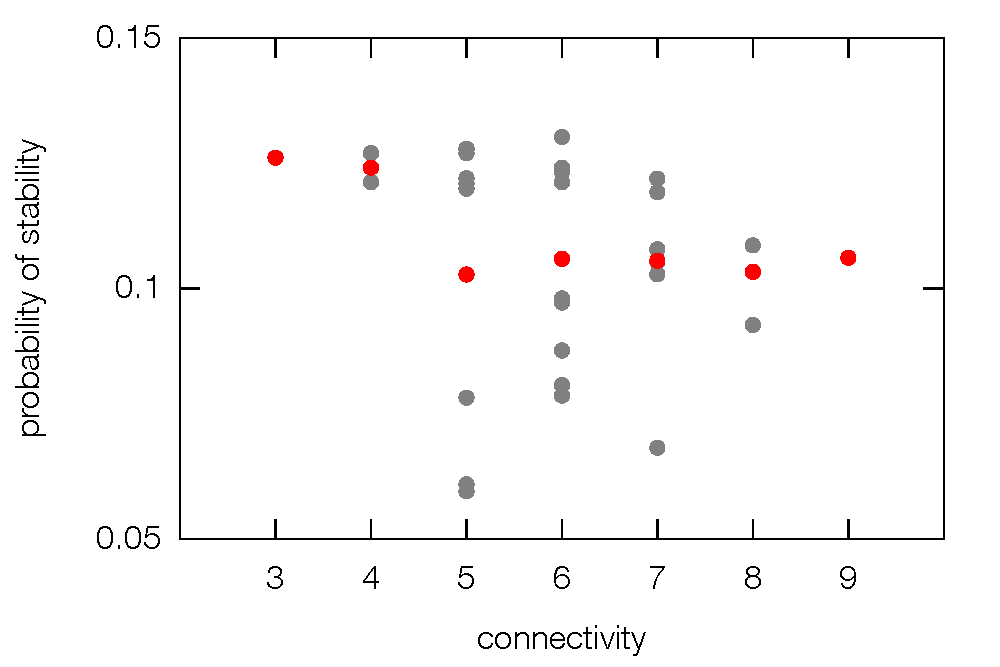
\includegraphics[width=0.8\columnwidth]{fig/apstab3x3.pdf}
% \caption{{\bf Plot of stability versus connectivity for three component systems.} }
% \label{fig:apstab3x3}
% \end{figure}

% \begin{figure}[!ht]
% \centering
% \noindent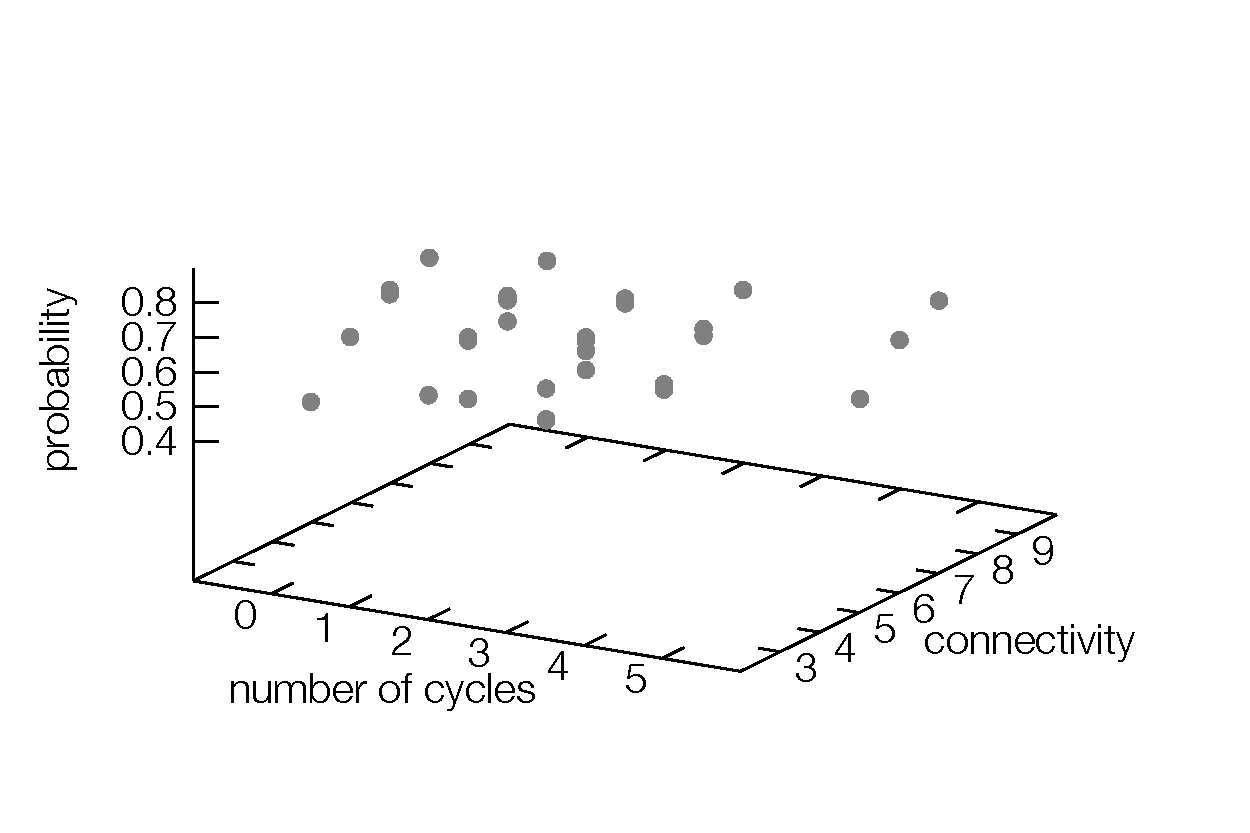
\includegraphics[width=0.8\columnwidth]{fig/connectcycle3D3x3.pdf}
% \caption{{\bf Plot of stability to perturbations versus number of cycles and connectivity for three component systems.} }
% \label{fig:connectcycle3D3x3}
% \end{figure}

% \begin{figure}[!ht]
% \centering
% \noindent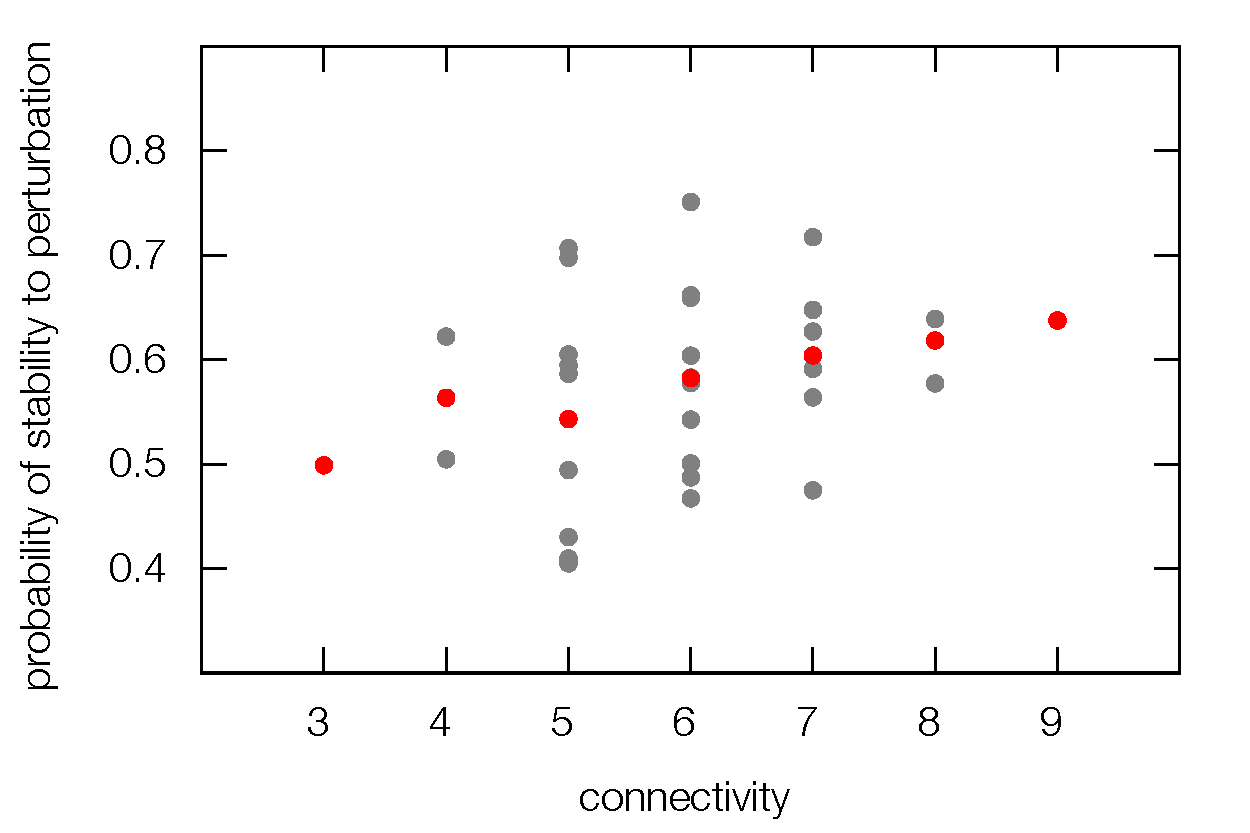
\includegraphics[width=0.8\columnwidth]{fig/stab3x3.pdf}
% \caption{{\bf Plot of stability to perturbations versus connectivity for three component systems.} }
% \label{fig:stab3x3}
% \end{figure}

% \begin{figure}[!ht]
% \centering
% \noindent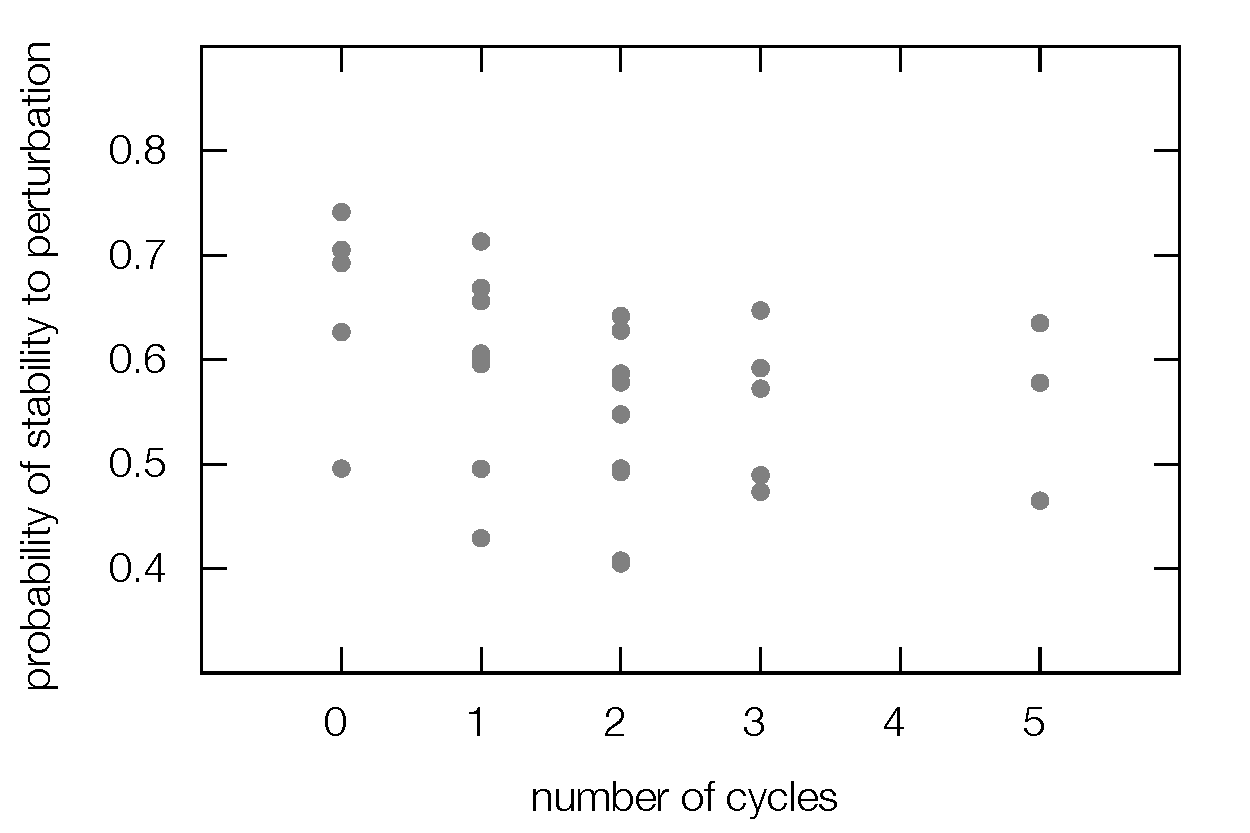
\includegraphics[width=0.8\columnwidth]{fig/cycle3x3.pdf}
% \caption{{\bf Plot of stability to perturbations versus number of cycles for three component systems.} }
% \label{fig:cycle3x3}
% \end{figure}
